% \iffalse meta-comment
%
% Copyright (C) 2010 by David Benjamin
% Copyright (C) 2012 by Benjamin Barenblat
%
% This file may be distributed and/or modified under the conditions of the
% LaTeX Project Public License, either version 1.2 of this license or (at your
% option) any later version.
%
% This file is distributed in the hope that it will be useful, but WITHOUT ANY
% WARRANTY; without even the implied warranty of MERCHANTABILITY or FITNESS
% FOR A PARTICULAR PURPOSE.  See the LaTeX Project Public License for more
% details.
%
% The latest version of the LaTeX Project Public License is in
%
%     http://www.latex-project.org/lppl.txt
%
% and version 1.2 or later is part of all distributions of LaTeX version
% 1999/12/01 or later.
%
% \fi
%
% \iffalse
%<*driver>
\ProvidesFile{6033dp1.dtx}
%</driver>
%
%<class>\NeedsTeXFormat{LaTeX2e}[1999/12/01]
%<class>\ProvidesClass{6033dp1}
%<*class>
    [2012/02/25 v1.0.0 MIT 6.033 design project]
%</class>
%
%<*driver>
\documentclass{ltxdoc}
\EnableCrossrefs
\CodelineIndex
\RecordChanges

\usepackage{eco}
\renewcommand{\sfdefault}{cmss}
\renewcommand{\ttdefault}{cmtt}

\usepackage{microtype}

\usepackage{hyperref}
\hypersetup{colorlinks,citecolor=blue}

\newcommand{\class}{\textsf{\jobname}}

%% Reference list is a section.  See
%% <http://stackoverflow.com/questions/1037905/bibliography-as-section-in-latex-bibtex>.
\newcommand{\bibname}{References}
\makeatletter
\renewenvironment{thebibliography}[1]
     {\section{\bibname}% <-- this line was changed from \chapter* to \section*
      \@mkboth{\MakeUppercase\bibname}{\MakeUppercase\bibname}%
      \list{\@biblabel{\@arabic\c@enumiv}}%
           {\settowidth\labelwidth{\@biblabel{#1}}%
            \leftmargin\labelwidth
            \advance\leftmargin\labelsep
            \@openbib@code
            \usecounter{enumiv}%
            \let\p@enumiv\@empty
            \renewcommand\theenumiv{\@arabic\c@enumiv}}%
      \sloppy
      \clubpenalty4000
      \@clubpenalty \clubpenalty
      \widowpenalty4000%
      \sfcode`\.\@m}
     {\def\@noitemerr
       {\@latex@warning{Empty `thebibliography' environment}}%
      \endlist}
\makeatother

\begin{document}
  \DocInput{6033dp1.dtx}
\end{document}
%</driver>
% \fi
%
% \CheckSum{330}
% \CharacterTable
% {Upper-case    \A\B\C\D\E\F\G\H\I\J\K\L\M\N\O\P\Q\R\S\T\U\V\W\X\Y\Z
%  Lower-case    \a\b\c\d\e\f\g\h\i\j\k\l\m\n\o\p\q\r\s\t\u\v\w\x\y\z
%  Digits        \0\1\2\3\4\5\6\7\8\9
%  Exclamation   \!     Double quote  \"     Hash (number) \#
%  Dollar        \$     Percent       \%     Ampersand     \&
%  Acute accent  \'     Left paren    \(     Right paren   \)
%  Asterisk      \*     Plus          \+     Comma         \,
%  Minus         \-     Point         \.     Solidus       \/
%  Colon         \:     Semicolon     \;     Less than     \<
%  Equals        \=     Greater than  \>     Question mark \?
%  Commercial at \@     Left bracket  \[     Backslash     \\
%  Right bracket \]     Circumflex    \^     Underscore    \_
%  Grave accent  \`     Left brace    \{     Vertical bar  \|
%  Right brace   \}     Tilde         \~}
%
% \changes{v1.0.0}{2012/02/25}{Initial release}
%
% \GetFileInfo{6033dp1.dtx}
%
% \DoNotIndex{\#,\$,\%,\&,\@,\\,\{,\},\^,\_,\~,\ }
% \DoNotIndex{\@ne}
% \DoNotIndex{\advance,\begingroup,\catcode,\closein}
% \DoNotIndex{\closeout,\day,\def,\edef,\else,\empty,\endgroup}
%
% \title{The \class\ class\thanks{%
%   This document corresponds to \class~\fileversion,%
%   dated~\filedate.}}
% \author{Benjamin Barenblat \\ \texttt{bbaren@mit.edu} \and David Benjamin \\ \texttt{davidben@mit.edu}}
%
% \maketitle
%
% \noindent \textsc{mit}'s 6.033 (Computer Systems Engineering) demands fairly specific formatting for design project assignments.
% This class adheres to those formatting conventions, as described in \cite{WAC09}.
%
% This class will not by default make your document look precisely like \cite{WAC09}.
% There is a \textsf{strict} option which will approach that style -- see section \ref{strictopt} -- but allowing \LaTeX\ to apply sensible defaults (rather than arbitrary ones, or even worse, those set by Microsoft Word) to your document will improve its design and readability significantly.
% Of course, the class's minimalism allows you great latitude in customizing the precise look and feel of your document.
%
% \section{Usage}
% \subsection{Enabling the class}
% You should specify |\documentclass{6033dp1}| at the start of your preamble.
% The class is based on \textsf{article}, so you can specify most of the optional arguments \textsf{article} can take; however, you cannot specify the \textsf{10pt} or \textsf{twocolumn} options, as 10-point or two-column text is explicitly disallowed by \cite{WAC09}.
% Additionally, \textsf{titlepage} is enabled by default; you can use \textsf{notitlepage} to disable it.
%
% \subsection{Additional metadata}
% \DescribeMacro{\recitation}
% In addition to the standard |\author|, |\date|, and |\title| commands, \class\ also provides the |\recitation| command.
% You should use it to specify information about your recitation, which will appear on the title page (or on the first page, if you have \textsf{notitlepage} set) after your name.
%
% \subsection{Tables}
% Tables are easily the most complicated case in this class.
% The class does a lot of styling to try to get them to look good, but it can't always get everything right.
% In particular, \class\ is unable to automatically insert grid lines in the tables you create; if you want them, you need to insert them yourself by placing pipes ($\vert$ characters) in |tabular| specifications and using the |\hline| command liberally throughout |tabular| bodies.
% For instance, you should set table 1 in \cite{WAC09} as
% \begin{quote}\begin{verbatim}
%\begin{table}[!h]
%  \caption{Heading Levels and Styles}
%  \begin{fulltabular}{|X|X|X|}
%    \hline
%    \thead{Unnumbered Headings} & \thead{Numbered Headings}\\
%    \hline
%    {\bfseries\Large Main Heading} &%
%                         {\bfseries\Large 1.0 Main Heading}\\
%    \hline
%    {\bfseries\large Second-Level Heading} &%
%                 {\bfseries\large 1.1 Second-Level Heading}\\
%    \hline
%    {\bfseries Third-Level Heading} &%
%                      {\bfseries 1.1.1 Third-Level Heading}\\
%    \hline
%    {\bfseries Another Third-Level Heading} &%
%              {\bfseries 1.1.2 Another Third-Level Heading}\\
%    \hline
%  \end{fulltabular}
%\end{table}
%\end{verbatim}\end{quote}
%
% This example depends several other \class-specific features.
% \DescribeMacro{\thead}
% For instance, \class\ defines the |\thead| macro as |\textbf{\textsc{|text|}}|.
% You should use it to identify table headings as required by \cite{WAC09}.
% \DescribeEnv{fulltabular}
% Additionally, this example uses the |fulltabular| environment, a simple wrapper around |tabularx| which is preset to the width of the text block.
% Thus, by specifying
% \begin{quote}\begin{verbatim}
%\begin{fulltabular}{|X|X|X|}
%\end{verbatim}\end{quote}
% this example defines a |tabularx| environment which will stretch to the width of the page and has three flexible left-aligned columns separated by vertical bars.
% (More information about |tabularx| specifications is provided in \cite{DC99}.)
%
% \subsection{Pseudocode}
% \class\ loads the \textsf{listings} package; you can thus place pseudocode in your document simply using the |lstlisting| environment:
% \begin{quote}\begin{verbatim}
%\begin{lstlisting}
%if(height > 60) {
%   cout << "You may ride this rollercoaster";
%} else {
%   cout << Maybe your older sibling will go with you";
%}
%\end{lstlisting}
%\end{verbatim}\end{quote}
%
% \subsection{Precise adherence to the style guide}
% \label{strictopt}
% If you really, really want your document to look as much like \cite{WAC09} as possible, you should specify the \textsf{strict} option.
% Furthermore, you should use \textsf{fulltabular} instead of any other table-making environment, and you should make sure to place lines in between all rows and columns.
% For example, table 2 in \cite{WAC09} is set as
% \begin{quote}\begin{verbatim}
%\begin{table}[!h]
%  \caption{Reported values for $a^2 + b^2$}
%  \label{reportedvalues}
%  \begin{fulltabular}{|X|X|X|}
%    $a$ & $b$ & $a^2 + b^2$\\
%    $1$ & $0$ & $1$\\
%    $2$ & $10$ & $103$\footnotemark[1]\\
%  \end{fulltabular}
%
%  \small\footnotemark[1] This value is suspect
%\end{table}
%\end{verbatim}\end{quote}
%
% You should also examine the example document in section \ref{styleguide}.
%
%
% \iffalse
%<*styleguide>
% \fi
%
%
% \section{Example document}
% \label{styleguide}
% Here is a copy of \cite{WAC09}, reset using this package.
%    \begin{macrocode}
\documentclass[strict]{6033dp1}

\title{Style Specification: A Guide to Formatting \\
  Conventions for the DP1 Report}
\author{Writing Across the Curriculum Staff}
\date{March 13, 2009}

\usepackage{graphicx}

\begin{document}
\maketitle

\section{Introduction and Overview}
Technical documents are judged by how completely, clearly, and quickly
they deliver information to a reader.  Skillful use of paragraphing,
sentence structure, and the proper use and definition of technical
terminology will help you create an informative document.  Careful
attention to the formatting of the report will improve its readability
and make information easier to find.

Most organizations that produce professional documents have a style
specification, style sheet, or other document that determines the
overall look of reports and other written material.  Although specific
conventions vary, guidelines help to ensure consistent format within a
particular community of writers.  The guidelines we use are based on
The Mayfield Handbook of Technical and Scientific Writing

\url{https://web.mit.edu/course/21/21.guide/www/home.htm}

For a complete discussion of any topic mentioned in this document,
follow the link to refer to the Mayfield Handbook.

\subsection{Global Document Format}
The following conventions allow you to give your report a professional
look and make information easy for the reader to find.  Writers can
achieve a clear, legible page layout using most generally available
text editing, word processing, or document production programs.

\begin{itemize}
\item Text should be single-spaced, left-justified (ragged right
  margin).  Leave one extra line space between paragraphs.
\item Use a single-column layout.
\item Font should be standard, 11- or 12-point.  You may use a second
  typeface or type style for headings, captions, and other special
  text.  Use these special effects sparingly.
\end{itemize}

\subsubsection{Headings}
Headings should stand out clearly from the running text of your
report.  \uline{Levels} of headings should be easy to identify; the
reader should easily distinguish high-level information from details
and examples.

You may indicate levels of headings through the use of type size and
style.  For a short document such as the DP1 report, which is limited
to 2500 words, too many levels of headings can be confusing.  Use just
\uline{three levels}.

Table~\ref{headingstyles} gives examples of the formatting styles for
three levels of section headings.

\begin{table}[!h]
  \caption{Heading Levels and Styles}
  \label{headingstyles}
  \begin{fulltabular}{|X|X|X|}
    \hline
    \thead{Unnumbered Headings} & \thead{Numbered Headings}\\
    \hline
    {\bfseries\Large Main Heading} &%
                         {\bfseries\Large 1.0 Main Heading}\\
    \hline
    {\bfseries\large Second-Level Heading} &%
                 {\bfseries\large 1.1 Second-Level Heading}\\
    \hline
    {\bfseries Third-Level Heading} &%
                      {\bfseries 1.1.1 Third-Level Heading}\\
    \hline
    {\bfseries Another Third-Level Heading} &%
              {\bfseries 1.1.2 Another Third-Level Heading}\\
    \hline
  \end{fulltabular}
\end{table}

For more information on headings, see:\\
\url{https://web.mit.edu/course/21/21.guide/www/headxsh.htm}

\subsection{Paragraphs and Logical Units of Information}
Readers of technical writing tend to skim documents, read them out of
order, and refer to sections that contain information they
particularly need.  Because readers have such a variety of styles of
using a document, they rely on writers to arrange information by topic
and to establish a clear progression of ideas.

If you craft a paragraph's first sentence carefully, that sentence can
establish context for the rest of the information in the paragraph and
announce the structure for presenting that information.  These first
sentences may be referred to as \uline{topic sentences},
contextualizing statements, or point sentences.  Spend extra time on
first sentences, and make sure that paragraphs are unified, focused,
and coherent.

Use \uline{bulleted and numbered lists} sparingly, and do not use them
to substitute for full discussions or explanations.  Lists should be
introduced with a short paragraph that explains and supplies context
for the items in the list.  Make sure that the items in the list
belong together and that they are grammatically parallel.

For example, you might begin each item with a boldface term and one or
more sentences explaining the term.  You might also list a series of
complete sentences or phrases that fit together logically.

For a complete discussion of topic sentences:\\
\url{https://web.mit.edu/course/21/21.guide/www/topic-s.htm}

For more information on the role of paragraphs and sentences, see:\\
\url{https://web.mit.edu/course/21/21.guide/www/paragraf.htm}\\
\url{https://web.mit.edu/course/21/21.guide/www/sentence.htm}

For more information on bulleted lists and other units of information,
see:\\
\url{https://web.mit.edu/course/21/21.guide/www/layout.htm}

\subsection{Guidelines for Graphics}
If you are not accustomed to using graphics to explain concepts, spend
some time looking at the illustrations in your course readings.  Which
graphics are helpful?  Which ones are confusing?  When students
critique the graphics they find in textbooks, manuals, and published
articles, they often complain that these illustrations are cluttered,
inaccurate, or difficult to relate to the concepts explained in
running text.  Give some thought to the specific point being made in
your graphic.  Adding captions, annotations, and figure numbers helps
readers to understand the point being made.

\subsubsection{Integrate graphics and text:}
\begin{itemize}
\item Summarize the intention of the graphic in the body text of your
  report.
\item Place the graphic as close as possible to a description of what
  it illustrates.
\item Use figure numbers and captions so that readers can switch
  attention between text and graphics easily.  Captions do count
  against your word limit, but readers often pay more attention to
  captions than to body text.
\end{itemize}

\begin{itemize}
\item The figure number and title belong under the figure.  You may
  put explanatory text after the figure title.

  For example, see the caption of Figure~\ref{samplefigure}.

  \begin{figure}[!h]
    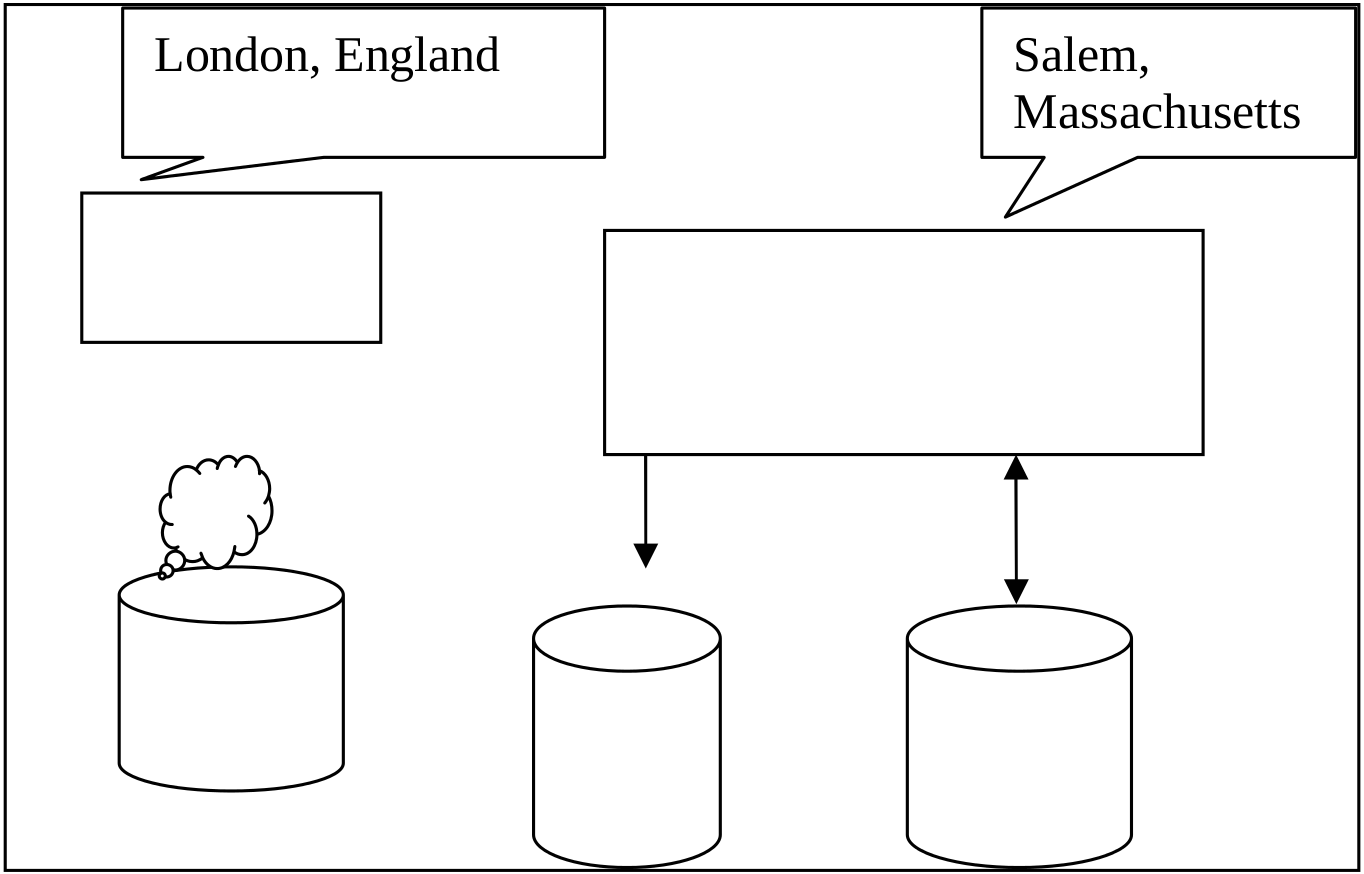
\includegraphics[width=4in]{figure1}
    \caption{A generic illustration.  Note that two unrelated place
      names are featured, and the cylinder on the left appears to be
      sulking.}
    \label{samplefigure}
  \end{figure}

\item In contrast, the table number and title belong \emph{on top of}
  the table, and explanatory text does \emph{not} follow the table
  title.  If necessary, concise explanatory notes may go in small type
  flush under the bottom of the table, as shown in
  Table~\ref{reportedvalues}.

\item Refer to visuals by number only, not position.  For example,
  write ``See Table \ref{reportedvalues}'' not ``See Table
  \ref{reportedvalues} \emph{below}.''

  \begin{table}[!h]
    \caption{Reported values for $a^2 + b^2$}
    \label{reportedvalues}
    \begin{fulltabular}{|X|X|X|}
      \hline
      $a$ & $b$ & $a^2 + b^2$\\
      \hline
      $1$ & $0$ & $1$\\
      \hline
      $2$ & $10$ & $103$\footnotemark[1]\\
      \hline
    \end{fulltabular}

    \small\footnotemark[1] This value is suspect
  \end{table}

\item Use a separate numbering scheme for tables and figures, as
  illustrated by Figure~\ref{samplefigure} and
  Table~\ref{reportedvalues}.  The next figure would be Figure~2, and
  the next table would be Table~III
\end{itemize}

\subsubsection{Emphasize the important detail:}
\begin{itemize}
\item Structure diagrams so important features are emphasized (e.g.,
  by position, labels, bold).  Avoid distracting lines, pictures, or
  special effects.
\item Label the axes of graphs, and specify the units of measurement
  you are using.
\end{itemize}

\subsubsection{Using Pseudocode}
You may use pseudocode examples, if they are kept brief and not used
as a substitute for prose explanations.  Remember that readers want to
see pseudocode as an illustration, but they will not want to decipher
a page of code to understand how your design works.  Pseudocode should
be formatted as a graphic and explained in the text of the report.
For example, the pseudocode in Figure~\ref{rollercoaster} illustrates
the use of 11-point Courier typeface to set it off from the rest of
the report's text, which is 12-point Times Roman.

\begin{figure}[!h]
\begin{lstlisting}
if(height > 60) {
   cout << "You may ride this rollercoaster";
} else {
   cout << Maybe your older sibling will go with you";
}
\end{lstlisting}
  \caption{Pseudocode for rollercoaster riders.}
  \label{rollercoaster}
\end{figure}

The example in Figure~\ref{emperors} shows additional hypothetical
code.  It provides a second illustration of 11-point Courier bold as
contrast with the report's running text:

\begin{figure}[!h]
  \begin{lstlisting}
while(ROME_BURNS) {
   fiddle;
}
  \end{lstlisting}
  \caption{Pseudocode for emperors.}
  \label{emperors}
\end{figure}

For more information on graphics, see:\\
\url{https://web.mit.edu/course/21/21.guide/www/grfxfig.htm}

\subsection{Footnotes}
\uline{Do not use footnotes} in the DP1 Report.  Consider the word
limit, and then weigh the value of any information you plan to include
against the space you have available.  If the information is
important, find a way to incorporate it into the report's running
text.  Bear in mind that any text included in footnotes counts against
the 2500-word limit.

To document your sources, use the IEEE style of in-text citation.  For
more information on IEEE citation, see:

\url{https://web.mit.edu/course/21/21.guide/www/doc-ie3.htm}
\end{document}
%    \end{macrocode}
% \iffalse
%</styleguide>
% \fi
% \setcounter{CodelineNo}{0}
%
%
% \section{License}
% \subsection{Class}
% The \class\ class is copyright \textcopyright\ 2010 by David Benjamin and 2012 by Benjamin Barenblat.
% You are free to distribute and/or modify it under the conditions of the \LaTeX\ Project Public License, either version 1.2 of this license or (at your option) any later version.
%
% This class is distributed in the hope that it will be useful, but \emph{without any warranty}; without even the implied warranty of \emph{merchantability} or \emph{fitness for a particular purpose}.
% See the \LaTeX\ Project Public License for more details.
%
% The latest version of the \LaTeX\ Project Public License is in
% \begin{quote}
%   \url{http://www.latex-project.org/lppl.txt}
% \end{quote}
% and version 1.2 or later is part of all distributions of \LaTeX\ version 1999/12/01 or later.
%
% \subsection{Example document}
% \cite{WAC09} is copyright \textcopyright\ 2009 by the Writing Across the Curriculum staff.
% All rights are reserved.
%
%
% \begin{thebibliography}{4}
% \bibitem{WAC09} Writing Across the Curriculum Staff, ``Style specifications: A guide to formatting conventions for the \textsc{dp}1 report,'' [Online document], 2009 Mar.\ 13, [cited 2012 Feb.\ 25], Available \textsc{http}: \url{http://web.mit.edu/6.033/2012/wwwdocs/dp1/DP1StyleGuide10.pdf}.
%
% \bibitem{DC99} D.~Carlisle, ``The \textsf{tabularx} package,'' [Online document], 1999 Jan.\ 7, [cited 2012 Feb.\ 25], Available \textsc{http}: \url{http://mirror.ctan.org/macros/latex/required/tools/tabularx.pdf}.
%
% \bibitem{LL07} L.~Lamport, F.~Mittelbach, J.~Braams, ``Standard document classes for \LaTeX\ version 2e,'' 2007 Oct.\ 19, Available as part of every \LaTeX\ distribution as |classes.pdf|.
%
% \bibitem{RMD02} R.~McDonnell, ``The \textsf{sectsty} package v2.0.2,'' [Online document], 2002 Feb.\ 25, [cited 2012 Feb.\ 25], Available \textsc{http}: \url{http://mirror.ctan.org/macros/latex/contrib/sectsty/sectsty.pdf}.
% \end{thebibliography}
%
%
% \StopEventually{\PrintIndex}
%
%
% \iffalse
%<*class>
% \fi
%
% \section{Implementation}
% \subsection{Options and base class}
% The \class\ class, being a technical document without part or chapter breaks, is based on the \textsf{article} class.
% I first define my options, and then I load the base class.
%
% \subsubsection{The title page}
% Design projects can have a title page, or it can be disabled (as for a project proposal).
%    \begin{macrocode}
\newif\ifdp@titlepage
\DeclareOption{titlepage}{\dp@titlepagetrue}
\DeclareOption{notitlepage}{\dp@titlepagefalse}
%    \end{macrocode}
%
% \subsubsection{Columns}
% Only one column is permitted, so trap attempts to use \textsf{twocolumn}.
%    \begin{macrocode}
\DeclareOption{twocolumn}{\ClassError{6033dp1}%
  {Two-column layout is not permitted}{}}
%    \end{macrocode}
%
% \subsubsection{Font}
% Only 11- or 12-point font is acceptable, so trap attempts to use \textsf{10pt}.
%    \begin{macrocode}
\DeclareOption{10pt}{\ClassError{6033dp1}%
  {10-point font is not permitted}{}}
%    \end{macrocode}
%
% \subsubsection{Precise adherence to \cite{WAC09}}
% If you really, really want your document to look as much as \cite{WAC09} as possible, you can specify the \textsf{strict} option.
%    \begin{macrocode}
\newif\ifdp@strict
\DeclareOption{strict}{\dp@stricttrue}
\DeclareOption{nostrict}{\dp@strictfalse}
%    \end{macrocode}
%
% \subsubsection{Other options}
% Any options that aren't explicitly defined for \class\ get passed on to \textsf{article}.
%    \begin{macrocode}
\DeclareOption*{\PassOptionsToClass{\CurrentOption}{article}}
%    \end{macrocode}
%
% \subsubsection{Default options}
% By default, the title page is turned on, precise adherence to \cite{WAC09} is disabled, and 11-point font is the default.
%    \begin{macrocode}
\ExecuteOptions{titlepage,nostrict}
\ProcessOptions\relax
\PassOptionsToClass{11pt}{article}
%    \end{macrocode}
%
% \subsubsection{Base class}
% Having defined and executed options, I can now load the base class.
%    \begin{macrocode}
\LoadClass{article}
%    \end{macrocode}
%
% \subsection{Metadata}
% \begin{macro}{\recitation}
% In addition to the standard author, title, and date metadata, design projects also may include a recitation section.
%    \begin{macrocode}
\newcommand*{\recitation}[1]{\gdef\@recitation{#1}}
%    \end{macrocode}
% The recitation section, if defined, is included on the title page.
% \end{macro}
%
% \subsection{The title page}
%
% If a title page is used, it contains the title and author-recitation-date block spaced evenly down the page.
% This code is modified from \cite{LL07}, section 7.1.
%    \begin{macrocode}
\ifdp@titlepage
  \renewcommand{\maketitle}{\begin{titlepage}%
      \let\footnotesize\small
      \let\footnoterule\relax
      \let \footnote \thanks
      \null\vfil
%    \end{macrocode}
% The title is centered and set in 14-point bold.
%    \begin{macrocode}
      \begin{center}%
        {\bfseries\large\@title}%
      \end{center}
      \vfil
%    \end{macrocode}
% The author-recitation-date block is set in normal body type and heavily indented down the page.
%    \begin{macrocode}
      \null\hspace{0.67\textwidth}%
        \parbox{0.33\textwidth}{\raggedright%
          \@author\\
          \ifx\@recitation\undefined\else{\@recitation\\}\fi
          \@date}
      \vfil
      \@thanks
    \end{titlepage}%
    \setcounter{footnote}{0}%
    \global\let\thanks\relax
    \global\let\maketitle\relax
    \global\let\@thanks\@empty
    \global\let\@author\@empty
    \global\let\@recitation\@empty
    \global\let\@date\@empty
    \global\let\@title\@empty
    \global\let\title\relax
    \global\let\author\relax
    \global\let\recitation\relax
    \global\let\date\relax
    \global\let\and\relax}
%    \end{macrocode}
%
% If no title page is used, the first page contains the title and author-recitation-date block.
%    \begin{macrocode}
\else
  \renewcommand{\maketitle}{\par
  \begingroup
    \renewcommand\thefootnote{\@fnsymbol\c@footnote}%
    \def\@makefnmark{\rlap{\@textsuperscript{\normalfont\@thefnmark}}}%
    \long\def\@makefntext##1{\parindent 1em\noindent
            \hb@xt@1.8em{%
                \hss\@textsuperscript{\normalfont\@thefnmark}}##1}%
    \newpage
    \global\@topnum\z@   % Prevents figures from going at top of page.
    \null
    \vskip 2em
    \begin{center}
      {\LARGE\bfseries\@title}
      \vskip 1.5em
      {\Large\lineskip .5em%
        \begin{tabular}[t]{c}%
          \@author
          \ifx\@recitation\undefined
          \else
          \\\@recitation
          \fi
        \end{tabular}\par}%
      \vskip 1em%
      {\large \@date}%
    \end{center}
    \thispagestyle{plain}\@thanks
  \endgroup
  \setcounter{footnote}{0}%
  \global\let\thanks\relax
  \global\let\maketitle\relax
  \global\let\@maketitle\relax
  \global\let\@thanks\@empty
  \global\let\@author\@empty
  \global\let\@date\@empty
  \global\let\@title\@empty
  \global\let\title\relax
  \global\let\author\relax
  \global\let\date\relax
  \global\let\and\relax
  }
\fi
%    \end{macrocode}
%
% \subsection{Global document format}
% Text is single-spaced and ragged-right.
% One extra line space goes between paragraphs.
%    \begin{macrocode}
\raggedright
\RequirePackage{parskip}
%    \end{macrocode}
%
% Pages have no heading, but they do have a running foot with the page number.
%    \begin{macrocode}
\RequirePackage{fancyhdr}
\pagestyle{fancy}
\fancyhf{}
\rfoot{\thepage}
\renewcommand{\headrulewidth}{0pt}
\renewcommand{\footrulewidth}{0pt}
%    \end{macrocode}
%
% \subsection{Section headers}
% Section headers are slightly different than those provided by the default \textsf{article} class.
% I'll use the \textsf{titlesec} package to style them correctly.
%
%    \begin{macrocode}
\RequirePackage{titlesec}
%    \end{macrocode}
%
% All section headings should have one em of space above them and no space between them and the body text.
%    \begin{macrocode}
\titlespacing*{\section}{0pt}{0.5em}{-0.5em}
\titlespacing*{\subsection}{0pt}{0.5em}{-0.5em}
\titlespacing*{\subsubsection}{0pt}{0.5em}{-0.5em}
%    \end{macrocode}
%
% \subsubsection{Top-level sections}
% Main headings (set with the |\section| macro) are set in 16-point bold.
% This is the default for the \textsf{article} class, so no adjustment is required.
% However, numbered sections are numbered as ``1.0'', not just ``1''.
%
% This hack appears in \cite{RMD02}, section 8.4.2.
%    \begin{macrocode}
\def\@seccntformat#1{\@ifundefined{#1@cntformat}%
  {\csname the#1\endcsname\quad}
  {\csname #1@cntformat\endcsname}
}
\def\section@cntformat{\thesection.0\quad}
%    \end{macrocode}
%
% \subsubsection{Subsections}
% Second-level headings (set with the |\subsection| macro) are set in 14-point bold.
% This is the default for the \textsf{article} class, so no adjustment is required.
%
% \subsubsection{Third-level sections}
% Third-level headings (set with the |\subsubsection| macro) are set in 12-point bold.
% This is the default for the \textsf{article} class, so no adjustment is required.
%
% \subsubsection{Other structure commands}
% Paragraph headings are not permitted.
%    \begin{macrocode}
\global\let\paragraph\undefined
\global\let\subparagraph\undefined
\global\let\subsubparagraph\undefined
%    \end{macrocode}
%
% \subsection{Tables}
% Table captions are set in 11-point bold.
% A period goes between the table number and the caption, and the caption is left-justified.
%    \begin{macrocode}
\RequirePackage[font={small,bf},labelsep=period,%
  justification=RaggedRight,%
  singlelinecheck=false]{caption}
%    \end{macrocode}
%
% Table numbers are set in Roman numerals.
%    \begin{macrocode}
\usepackage[T1]{fontenc}
\renewcommand{\thetable}{\Roman{table}}
%    \end{macrocode}
%
% \begin{macro}{\thead}
% Column headings are set in bold small caps.
%    \begin{macrocode}
\newcommand{\thead}[1]{\textbf{\textsc{#1}}}
%    \end{macrocode}
% \end{macro}
%
% Footnotes in |table| environments should be ordered as {\renewcommand\thefootnote{\fnsymbol{footnote}}\footnotemark[1], \footnotemark[2], etc.}
%    \begin{macrocode}
\let\Table\table
\renewcommand{\table}[1][1]{\Table[#1]%
  \renewcommand\thefootnote{\fnsymbol{footnote}}}
%    \end{macrocode}
%
% \begin{environment}{fulltabular}
% It's occasionally useful -- especially if you're trying to emulate the style in \cite{WAC09} as closely as possible -- to have a table span the entire page width, so I define a second |tabularx| wrapper which does just this.
%    \begin{macrocode}
\RequirePackage{tabularx}
\newenvironment{fulltabular}[1]{%
  \tabularx{\textwidth}{#1}}{%
  \endtabularx}
%    \end{macrocode}
% \end{environment}
%
% \subsection{Code}
% Code is typeset in bold teletype text.
%    \begin{macrocode}
\RequirePackage{listings}
\lstset{basicstyle=\bfseries\ttfamily\small}
%    \end{macrocode}
%
% \subsection{Footnotes}
% \cite{WAC09} forbids the use of footnotes.
%    \begin{macrocode}
\renewcommand{\footnote}{\ClassError{6033dp1}%
  {Footnotes are not permitted}{}}
%    \end{macrocode}
%
% \subsection{Strict adherence to \cite{WAC09}}
% If \textsf{strict} was set, then a whole bunch of things happen.
%    \begin{macrocode}
\ifdp@strict
%    \end{macrocode}
%
% \subsubsection{Fonts}
% The font scheme gets set to Times, Helvetica, and Courier.
%    \begin{macrocode}
  \RequirePackage{txfonts}
  \RequirePackage[scaled]{helvet}
  \RequirePackage{courier}
%    \end{macrocode}
%
% \subsubsection{Section headers}
% All section headers have numbering disabled.
%    \begin{macrocode}
  \setcounter{secnumdepth}{0}
%    \end{macrocode}
%
% \subsubsection{Lists}
% Spacing within lists is severely reduced.
%    \begin{macrocode}
  \let\Itemize\itemize
  \renewcommand{\itemize}{\Itemize\setlength{\itemsep}{-0.67em}}
  \let\Enumerate\enumerate
  \renewcommand{\enumerate}{\Enumerate\setlength{\itemsep}{-0.67em}}
%    \end{macrocode}
%
% \subsubsection{Hyperlinks}
% Hyperlinks within the document are not distinguished in any special way; hyperlinks outside the document are blue.
%    \begin{macrocode}
  \RequirePackage[normalem]{ulem}
  \RequirePackage[dvipdfm]{hyperref}
  \hypersetup{colorlinks,linkcolor=black,urlcolor=blue}
%    \end{macrocode}
% Additionally, all hyperlinks are set in roman (not teletype) font.
%    \begin{macrocode}
  \def\UrlFont{\rmfamily}
  \def\UrlLeft{\uline\bgroup}
  \def\UrlRight{\egroup}
%    \end{macrocode}
%
%    \begin{macrocode}
\fi
%    \end{macrocode}
%
% \iffalse
%</class>
% \fi
%
% \Finale
%
\endinput
